\documentclass[12pt]{report}
\usepackage{./sty/dissert}% style
\usepackage{comment}
\usepackage[acronym]{glossaries}
\usepackage{titlesec}
\usepackage{xcolor}
\usepackage{amsmath}
\usepackage{tikz}
\usepackage{float}
\usetikzlibrary{calc,positioning}
\hypersetup{
    colorlinks,
    linkcolor={black!50!black},
    citecolor={black!50!black},
    urlcolor={black!80!black}
}
\titleformat{\chapter}{\LARGE}{\thechapter.}{20pt}{\LARGE\textbf}
\titlespacing*{\chapter}{0pt}{0pt}{20pt}
\renewcommand{\figurename}{Figura}
\titleformat*{\section}{\large\bfseries}
%
\makeglossaries%
 % ------------------- Document -----------------------------------------------------
\begin{document}
%\onehalfspacing
\pagenumbering{roman}
\newcommand\tab[1][1cm]{\hspace*{#1}}
% title page
\begin{titlepage}

\newcommand{\HRule}{\rule{\linewidth}{0.5mm}} % Defines a new command for the horizontal lines, change thickness here

\center % Center everything on the page
 %    LOGO SECTION

\FloatBarrier
\begin{figure}[ht!]
    \centering
    %\captionsetup{justification=centering,margin=2cm}
    
\includegraphics[width=0.4\textwidth]{img/logo.png}  
\end{figure}
\FloatBarrier
\vspace{0.5cm}

%    HEADING SECTIONS

{\LARGE Universidade do Minho}\\[0.5cm] % Name of your university/college
{\Large Escola de Engenharia}\\[0.5cm] % Name of your university/college
{\Large Mestrado em Engenharia Eletrónica Industrial e Computadores}\\[0.5cm] % Major heading such as course name

{\Large  Sistemas Autónomos Inteligentes}\\%[0.5cm] % Minor heading such as course title

%------------------------------------------------------------------------------------
%    TITLE SECTION

 {\large\emph{}}\\[0.5cm]
\HRule \\[0.3cm]

{\LARGE   \bfseries \scshape Relatório de Cinemática 
}
\HRule \\[0.3cm]

%------------------------------------------------------------------------------------
%    AUTHOR SECTION

\vspace{0.1cm} %5mm vertical space
\Large{Autores:}\\
\vspace{0.3cm} %5mm vertical space
\begin{tabular}{ll}
    Fábio Pereira Alves & PG6\\
    Lara Fernandes & PG63895\\
    Nádia Silva & PG63900\\
    Nuno Costa & PG63901\\
   
  \end{tabular}%
\\[1cm] % Your name

%------------------------------------------------------------------------------------
%    ACADEMIC ADVISORS SECTION

%\vspace{0.1mm} %5mm vertical space
Professora:\\
\vspace{0.3cm} %5mm vertical space
\begin{tabular}{ll}
    Estela Bicho\\

  \end{tabular}%
  \\[0.3cm] % Your name
%------------------------------------------------------------------------------------
%    DATE SECTION
%{\large \textsc{\today}}
%\vfill 
%\pagenumbering{arabic}
\end{titlepage}
%\pagenumbering{arabic}
\newpage
\newacronym{eeic}{EEIC}{Engenharia Eletrónica Industrial e de Computadores}
\newacronym{um}{UM}{Universidade do Minho}
%
% --------------Indices------------------
\renewcommand{\contentsname}{Índice}
\renewcommand{\listfigurename}{Lista de Figuras}
\renewcommand{\listtablename}{Lista de Tabelas}
\tableofcontents
\newpage
\listoffigures
\newpage
%
\phantomsection%
%\addcontentsline{toc}{chapter}{Índice}
%\printglossary[type=\acronymtype,title=Lista de Abreviações]
\cleardoublepage%
%
% --------------TRABALHO------------------
\renewcommand\chaptername{Capítulo}
%----- INTRODUÇÃO -----------
\pagenumbering{arabic}
%
%
\chapter{Introdução}
\label{ch:intro}
%
%
%
\section{Resumo}
\label{sec:resumo}
%
Este projeto consiste no desenvolvimento de um robô autónomo capaz de detetar obstáculos e afastar-se deles, à medida que se aproxima do alvo pretendido. Para a criação deste robô, foi necessário seguir uma determinada ordem de trabalhos para obter o produto final. 

Primeiramente, foi necessário o desenvolvimento do modelo do robô, recorrendo-se a uma ferramenta CAD (Autodesk Fusion 360). Nesta plataforma, foram concebidas as diferentes peças que constituem o modelo do robô.  

De seguida, todas as peças em CAD foram importadas da plataforma para o CoppeliaSim, de forma a criar o modelo físico do robô.  

Por fim, para a navegação autónoma, foram implementados os algoritmos baseados em sistemas dinâmicos não lineares em Matlab e também foi realizada a comunicação entre o Matlab e o CoppeliaSim para o controlo do robô.
\section{Enquadramentos e objetivos}
\label{sec:enq-e-obj}
%
No âmbito da Unidade Curricular de Sistemas Autónomos Inteligentes do curso de Mestrado em Engenharia Eletrónica Industrial e Computadores da Universidade do Minho, desenvolveu-se um robô autónomo capaz de detetar obstáculos e afastar-se deles, à medida que se aproxima do alvo pretendido. Pretendeu-se desta forma conciliar os conhecimentos adquiridos nas diferentes unidades curriculares da especialização de Controlo, Automação e Robótica e utilizá-los no desenvolvimento do projeto. 

O objetivo concreto deste projeto passou, então, por desenvolver um robô desde a sua raiz, criando e/ou escolhendo todas as peças constituintes deste. Este robô tem de ser capaz de se movimentar fazendo uma trajetória completamente autónoma, tendo apenas como conhecimento inicial as coordenadas do alvo final. Durante este trajeto até ao alvo, o robô tem de ser capaz de agir conforme as situações a que poderá vir a ser sujeito, tais como a presença de obstáculos na sua trajetória ou até mesmo alteração em tempo real da posição do alvo.  

Tendo isto em conta, para o desenvolvimento do robô é possível identificar os seguintes tópicos:

\begin{itemize}
\item Esboço e definição de medidas das várias peças do robô;
\item Escolha e pesquisa das peças que constituem o robô;
\item Desenvolvimento do modelo do robô com uso da ferramenta CAD;
    \begin{itemize}
        \item Criação do modelo físico da plataforma em CoppeliaSim; 
        \item Adaptação dos scripts Matlab para controlo do novo robô;
    \end{itemize}
\item Navegação autónoma:
    \begin{itemize}
        \item -Implementação de algoritmos para a navegação autónoma baseados em sistemas dinâmicos não-lineares;
        \item Desenvolvimento de um programa em Matlab e comunicação entre Matlab e CoppeliaSim para o controlo do robô; 

 
    \end{itemize}
\end{itemize}
\setcounter{table}{0}
\setcounter{figure}{0}

\input{tex/Chap/2-Direct_Kin/DIR_KIN}
\setcounter{table}{0}
\setcounter{figure}{0}

\input{tex/Chap/3-Inverse_kin/INV_KIN}
\setcounter{table}{0}
\setcounter{figure}{0}

\chapter{Implementação em MATLAB}
\label{ch:matlab}

Neste subcapítulo, são apresentados os resultados obtidos após a junção do modelo físico do robô, elaborado no CoppeliaSim, com as alterações efetuadas no código Matlab.

\section{Resultados}
\label{sec:resultados}

Para isso, realizaram-se vários testes de forma a obter-se o desempenho pretendido, ou seja, um robô capaz de navegar autonomamente até a um ou mais alvos num cenário que contém obstáculos. Nas figuras seguintes pode-se comprovar que se alcançou o comportamento desejado.

        %
    \begin{figure}[!h] 
\centering
    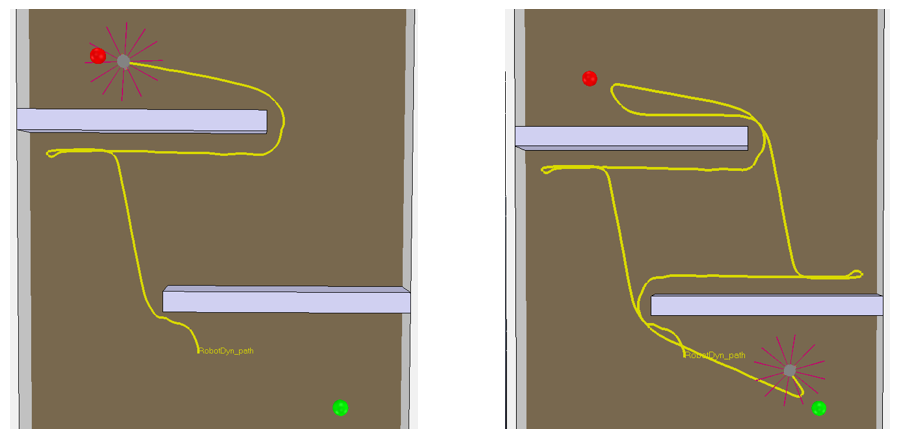
\includegraphics[width=0.9\textwidth]{./img/trajetoria}
  \caption{Trajetória para o alvo vermelho (esquerda) e para o verde (direita)}
  %
\label{fig:traj}
\end{figure}

O robô tinha como destino inicial o alvo representado pela esfera vermelha. Para lá chegar deparou-se com dois obstáculos. Quando um obstáculo é detetado, a velocidade do robô diminui de modo que este tenha uma resposta eficaz no desvio do obstáculo, evitando a colisão com o mesmo. Sendo assim, na figura da esquerda, confirma-se que o robô se desviou com sucesso, conseguindo, por fim, alcançar o alvo. Após esse momento, o robô encontrou-se pronto para seguir para o próximo alvo, representado pela esfera de cor verde, onde mais uma vez teve de contornar os obstáculos detetados pelos sensores, e alterar a velocidade, conforme a situação em que se encontrava, durante o seu percurso até chegar ao alvo pretendido, como se vê na figura da direita. Também na figura da direita, pode-se observar toda esta trajetória que o robô desempenhou sendo que, neste caso, o seu destino mudava de um alvo para o outro sempre que um deles era alcançado.

Obtido o desempenho pretendido para o projeto, prosseguiu-se com a adição extra de um robô. O objetivo é que este siga o robô principal pois, para o novo robô, esse é o seu alvo. Sendo assim, o segundo robô tem que acompanhar a trajetória que o primeiro robô executa em direção a um dos alvos. Os resultados obtidos podem ser vistos nas figuras seguintes.

        %
    \begin{figure}[!h] 
\centering
    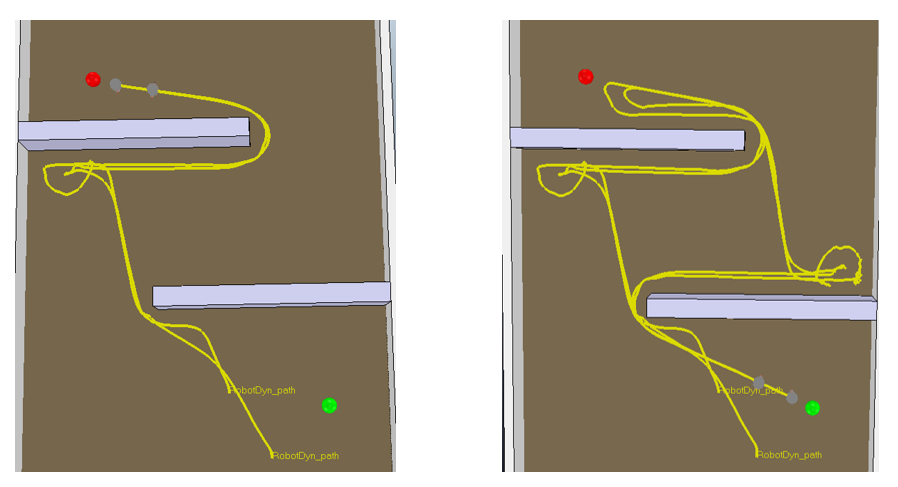
\includegraphics[width=0.9\textwidth]{./img/trajetoria-2}
  \caption{Trajetória dos dois robôs para o alvo vermelho (esquerda) e para o verde (direita)}
  %
\label{fig:traj-2}
\end{figure}

Tal como no caso anterior, o destino inicial era o target vermelho e tanto o robô principal como o secundário tiveram que se desviar dos dois obstáculos para chegarem ao destino. O procedimento para o fazerem foi o mesmo que o do teste com apenas um robô mencionado em cima. Ainda é de referir que o segundo robô também deteta os obstáculos e a velocidade dos dois robôs também se ajusta perante a situação em que se encontram. O segundo robô mantém sempre uma distância de 60 cm do primeiro robô para evitar colisões entre eles. Com estas condições, o primeiro robô quando encontra um obstáculo e uma parede lateral tem mais dificuldade em sair desse local visto que o segundo robô também é considerado um obstáculo para o primeiro. No entanto, consegue desviar-se e seguir a sua rota para qualquer um dos targets, vermelho ou verde, tal como no caso anterior.
\section{Discussão}
\label{sec:disc}

Obtidos os resultados, far-se-á, neste capítulo, uma análise dos mesmos de forma a entender o comportamento do robô em cada situação.

Começando pelo cenário em forma de S e com apenas um robô, quando o robô deteta um obstáculo, a força repulsiva do obstáculo torna-se cada vez mais forte à medida que mais sensores detetam obstáculos virtuais e sobrepõe-se à força atrativa do alvo. Dá-se, nesse momento, uma bifurcação onde o ponto fixo atrator que atraía o robô na direção do alvo, altera-se para um repulsor, logo o robô responde, afastando-se do obstáculo. Como de cada lado do repulsor existe um atrator, há duas possibilidades, virar à esquerda ou virar à direita. A escolha entre essas duas possibilidades depende da bacia de atração em que a direção de navegação fica no momento da bifurcação.

À medida que o robô se move, a informação sensorial varia e, por conseguinte, os atratores e os repulsores deslocam-se. Sendo assim, o controlo da velocidade é fulcral para manter o sistema estável, ou seja, num, ou perto de um, atrator. Para isso, a velocidade de translação do robot deve ser controlada de forma que a velocidade com que os atractores se deslocam seja inferior à velocidade de relaxamento da dinâmica da direção de navegação. 

Quando nenhuma obstrução é detetada, a velocidade do robô é estabilizada por um atrator cujo valor é proporcional à distância ao alvo, de acordo com a contribuição do alvo imposta pela função potencial. Quando são detetadas obstruções, o valor de intensidade da força de atração do obstáculo é positivo para o valor corrente da direção de navegação, e neste caso, a dinâmica de velocidade é governada por um atrator que é especificado pelas contribuições dos obstáculos. Todavia, quando são detetadas obstruções, mas a direção de navegação do robô fica fora da zona repulsiva criada pelas obstruções, a dinâmica da velocidade é dominada pela contribuição do alvo e o robô acelera novamente.

Para analisar se as contribuições dos obstáculos estão presentes, integram-se as forças de repulsão dos obstáculos o que resulta numa função potencial do sistema dinâmico que gera o comportamento “evitar colisões com obstáculos”. Valores positivos desta função indicam que a direção de navegação está dentro duma zona repulsiva, criada pelos obstáculos, pelo que é necessário ter a intensidade de atração do obstáculo maior que 0 e a intensidade de atração do alvo igual a 0. Reciprocamente, valores negativos do potencial indicam que a direção de navegação está fora da zona repulsiva ou então que as forças repulsivas dos obstáculos são fracas, daí que a intensidade de atração do obstáculo igual a 0 e a intensidade de atração do alvo maior que 0 seja necessário neste caso. A seguinte hierarquia de taxas de relaxação assegura que o todo o sistema converge para os atractores e que o comportamento “evitar obstáculos” tem prioridade sobre o comportamento “movimento na direção do alvo”:
        %
    \begin{figure*}[!h] 
\centering
    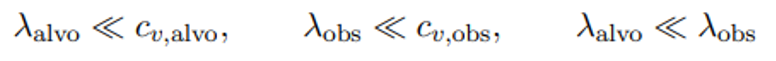
\includegraphics[width=0.7\textwidth]{./img/conc}
  %
\label{fig:traj-2}
\end{figure*}

Os testes feitos, para o caso de apenas um robô, foram acompanhados de gráficos dinâmicos que se iam alterando conforme a situação em que o robô se encontrava. Observa-se nesses gráficos a força atrativa do alvo, a dinâmica resultante das contribuições do alvo e obstáculos e, por último, a força dos obstáculos e a função potencial. Através das suas análises, confirma-se que o gráfico da força atrativa do alvo mostra, com o declive negativo, o ponto fixo atrator que atrai o sistema para o valor que ele especifica e um ponto fixo repulsor com o declive positivo na direção oposta à direção onde se localiza o alvo. Verifica-se, também, que a força repulsiva dos obstáculos aumenta quando mais sensores detetam o obstáculo e a distância diminui. Quanto ao gráfico da dinâmica total, quando já não é necessário que o robô se desvie de um obstáculo, a dinâmica da direção de navegação forma um atractor na direção que aponta para o alvo. Inversamente, a dinâmica da direção de navegação edifica um repulsor nessa direção quando se tem que desviar do obstáculo. Finalmente, a função potencial resulta do integral da força repulsiva que é máxima perto da direção onde se localiza o obstáculo que tem que ser evitada. Quanto maior a força repulsiva, menor é a velocidade de translação do robô.

Quanto ao cenário em forma de S mas com os dois robôs, o comportamento do primeiro robô é justificado da mesma forma que o caso anterior. Já o segundo robô tem o robô que está à sua frente como o seu alvo, ou seja, um atrator, pelo que o seu comportamento altera-se conforme a situação que o primeiro robô enfrenta. No caso do robô secundário estar a detetar obstáculos,  as forças repulsivas predominam em relação à força atrativa do robô primário. Logo, deixa de seguir o primeiro robô e desvia-se do obstáculo seguindo a justificação dada anteriormente. Após ultrapassar o obstáculo, volta a seguir o robô.

\section{Resultados}
\label{sec:resultados}

Para isso, realizaram-se vários testes de forma a obter-se o desempenho pretendido, ou seja, um robô capaz de navegar autonomamente até a um ou mais alvos num cenário que contém obstáculos. Nas figuras seguintes pode-se comprovar que se alcançou o comportamento desejado.

        %
    \begin{figure}[!h] 
\centering
    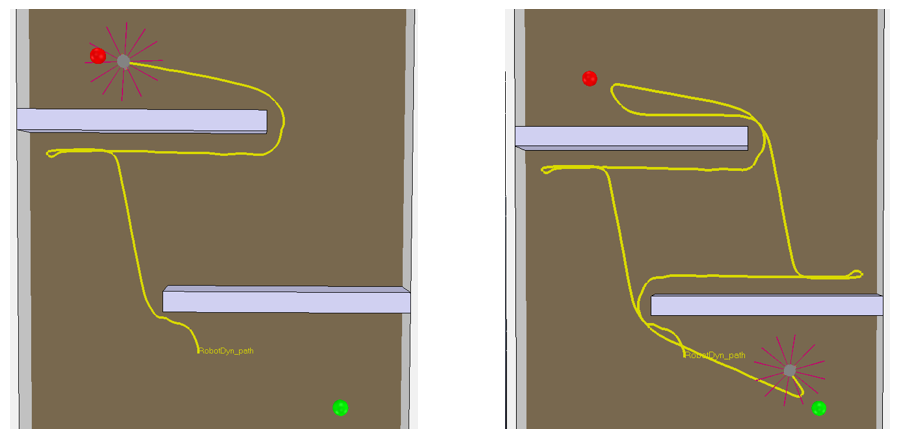
\includegraphics[width=0.9\textwidth]{./img/trajetoria}
  \caption{Trajetória para o alvo vermelho (esquerda) e para o verde (direita)}
  %
\label{fig:traj}
\end{figure}

O robô tinha como destino inicial o alvo representado pela esfera vermelha. Para lá chegar deparou-se com dois obstáculos. Quando um obstáculo é detetado, a velocidade do robô diminui de modo que este tenha uma resposta eficaz no desvio do obstáculo, evitando a colisão com o mesmo. Sendo assim, na figura da esquerda, confirma-se que o robô se desviou com sucesso, conseguindo, por fim, alcançar o alvo. Após esse momento, o robô encontrou-se pronto para seguir para o próximo alvo, representado pela esfera de cor verde, onde mais uma vez teve de contornar os obstáculos detetados pelos sensores, e alterar a velocidade, conforme a situação em que se encontrava, durante o seu percurso até chegar ao alvo pretendido, como se vê na figura da direita. Também na figura da direita, pode-se observar toda esta trajetória que o robô desempenhou sendo que, neste caso, o seu destino mudava de um alvo para o outro sempre que um deles era alcançado.

Obtido o desempenho pretendido para o projeto, prosseguiu-se com a adição extra de um robô. O objetivo é que este siga o robô principal pois, para o novo robô, esse é o seu alvo. Sendo assim, o segundo robô tem que acompanhar a trajetória que o primeiro robô executa em direção a um dos alvos. Os resultados obtidos podem ser vistos nas figuras seguintes.

        %
    \begin{figure}[!h] 
\centering
    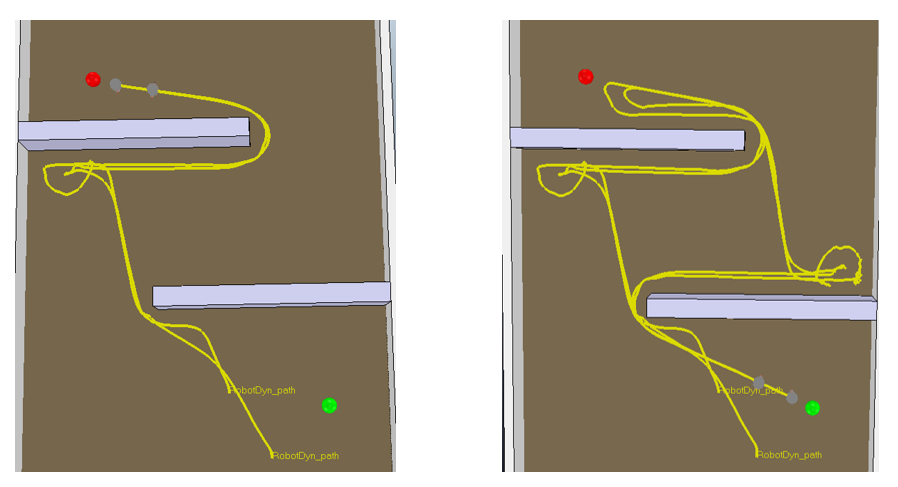
\includegraphics[width=0.9\textwidth]{./img/trajetoria-2}
  \caption{Trajetória dos dois robôs para o alvo vermelho (esquerda) e para o verde (direita)}
  %
\label{fig:traj-2}
\end{figure}

Tal como no caso anterior, o destino inicial era o target vermelho e tanto o robô principal como o secundário tiveram que se desviar dos dois obstáculos para chegarem ao destino. O procedimento para o fazerem foi o mesmo que o do teste com apenas um robô mencionado em cima. Ainda é de referir que o segundo robô também deteta os obstáculos e a velocidade dos dois robôs também se ajusta perante a situação em que se encontram. O segundo robô mantém sempre uma distância de 60 cm do primeiro robô para evitar colisões entre eles. Com estas condições, o primeiro robô quando encontra um obstáculo e uma parede lateral tem mais dificuldade em sair desse local visto que o segundo robô também é considerado um obstáculo para o primeiro. No entanto, consegue desviar-se e seguir a sua rota para qualquer um dos targets, vermelho ou verde, tal como no caso anterior.
\setcounter{table}{0}
\setcounter{figure}{0}

\input{tex/Chap/5-Resultados/TEST}
\setcounter{table}{0}
\setcounter{figure}{0}

\chapter{Conclusão}
\label{ch:conc}

Através da realização deste projeto no âmbito da Unidade Curricular Sistemas Autónomos Inteligentes, desenvolveram-se técnicas e competências aprendidas durante o percurso universitário e conseguiu-se também entender de uma forma mais explícita e concreta como funciona o desenvolvimento de um projeto ligado à navegação autónoma de um robô.

Neste trabalho, criou-se um robô em CAD, numa plataforma nunca utilizada pelos elementos do grupo. Exportou-se esse robô para um ambiente de simulação, onde teve que passar por várias etapas até se obter um robô capaz de desempenhar uma navegação autónoma, através do uso do código que foi produzido e alterado de acordo com as características do robô e com o que se pretendia que ele fizesse. Por fim, ainda se adicionou mais um robô demonstrando que o código é adaptável e que se poderá futuramente ter uma série de robôs a navegar autonomamente e executando o mesmo trajeto. Uma outra sugestão consiste em testar o funcionamento destes robôs noutros cenários.

Pode-se assim afirmar que se enfrentaram algumas adversidades enquanto se desenvolvia o protótipo. Não obstante, tentou-se sempre encontrar soluções para resolver esses problemas e nos casos em que tal não foi possível, procurou-se sempre contorná-los. No final, obteve-se sucesso nos resultados alcançados visto que foram de encontro ao que era pretendido, tanto num robô como nos dois.

É de salientar ainda que todo o tempo utilizado por todos os membros do grupo foi gerido de forma a ser o mais proveitoso possível. 

Por último, são projetos como estes que colocam os alunos mais próximos do mundo do trabalho, uma vez que com a realização deste projeto, se sentiu que é fulcral recorrer-se às simulações para futuramente colocar-se em prática e obter-se um bom desempenho.

\setcounter{table}{0}
\setcounter{figure}{0}

\begin{thebibliography}{9}

\bibitem{aula_kin}
Apontamentos da unidade curricular, \textit{Basics of kinematics: 2 DOF planar arm} e \textit{3 DOF planar arm} (abordagem geométrica).

\bibitem{mycobot}
Elephant Robotics, \textit{myCobot 280: documentação}, \url{https://docs.elephantrobotics.com}.

\bibitem{coppelia}
Coppelia Robotics, \textit{CoppeliaSim User Manual: ZeroMQ remote API}, \url{https://manual.coppeliarobotics.com}.

\bibitem{matlab}
The MathWorks, \textit{MATLAB Documentation}, \url{https://www.mathworks.com/help/matlab/}.

\end{thebibliography}

\setcounter{table}{0}
\setcounter{figure}{0}
%\input{tex/Chap/INTRO} % Introduction
%\input{kalman_equations}
%\input{ANALYSIS} % Analysis of the problem
%\input{DESIGN} % Algorithms design and Workflow
%\input{EX1} % Matlab implementation
%\input{tex/Chap/NEURON-NO-SELF-EXCITATION} % EX1
%\input{tex/Chap/NEURON-SELF-EXCITATION} % EX2
%\input{tex/Chap/TWO-NEURONS} % EX3
%\input{tex/Chap/TARGET-SELECTION} % EX4
%\input{TESTS} % Testing
%\input{tex/Chap/CONCLUSION} % Conclusions and Future Work
%
% -------------- BIBLIO ---------------------
%\bookmarksetup{startatroot} % Ends last part.
%\bibliographystyle{unsrtnat}
%\renewcommand{\bibname}{Referências} 
%\bibliography{bib/dissert}


\end{document}
